\documentclass[tikz,border=5mm]{standalone}
\usetikzlibrary{arrows.meta, decorations.pathreplacing, calligraphy}

\begin{document}
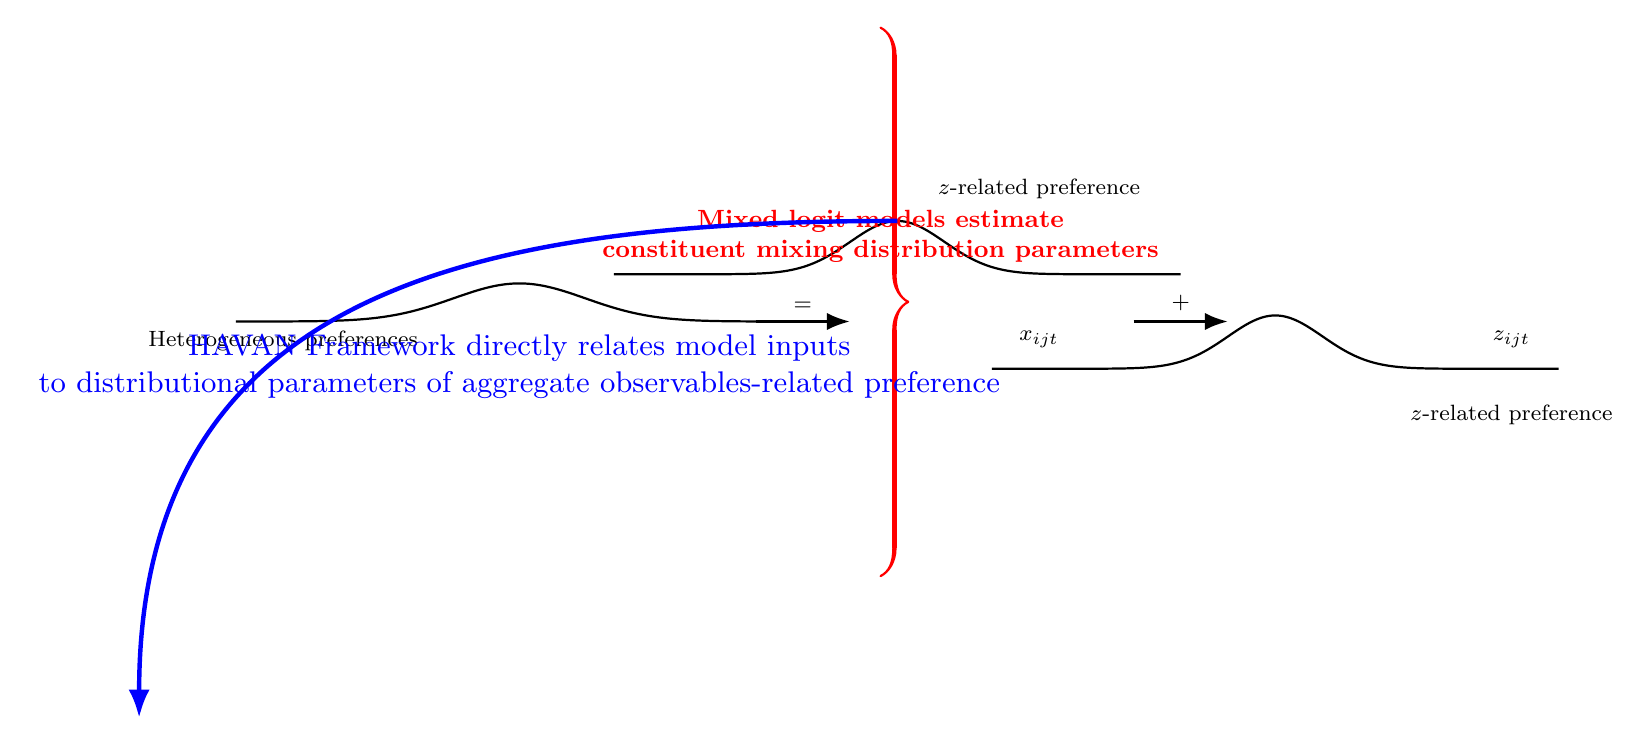
\begin{tikzpicture}[
    >=Latex,
    declare function={
        gaussian(\x,\m,\s) = 1/(2*\s*sqrt(pi))*exp(-(\x-\m)^2/(2*\s^2));
    },
    scale=1.2,
    every node/.style={font=\footnotesize},
]

% Define the Gaussian curve functions
\def\gaussOne{-3,-2,...,3}
\def\gaussTwo{-3,-2,...,3}

% Draw the first Gaussian curve (left side)
\foreach \x in \gaussOne {
    \pgfmathparse{gaussian(\x,0,0.7)}
    \coordinate (A\x) at (\x, \pgfmathresult);
}
\draw[thick, smooth] plot[variable=\x,samples=100,domain=-3:3] ({\x},{gaussian(\x,0,0.7)});
\node[below] at (-2.5,0) {Heterogeneous preferences};

% Draw the second Gaussian curve (middle)
\foreach \x in \gaussTwo {
    \pgfmathparse{gaussian(\x,0,0.5)+0.5}
    \coordinate (B\x) at (\x+4, \pgfmathresult);
}
\draw[thick, smooth] plot[variable=\x,samples=100,domain=-3:3] ({\x+4},{gaussian(\x,0,0.5)+0.5});
\node[below] at (5.5,0) {$x_{ijt}$};
\node[above] at (5.5,1.2) {$z$-related preference};

% Draw the third Gaussian curve (right)
\foreach \x in \gaussTwo {
    \pgfmathparse{gaussian(\x,0,0.5)-0.5}
    \coordinate (C\x) at (\x+8, \pgfmathresult);
}
\draw[thick, smooth] plot[variable=\x,samples=100,domain=-3:3] ({\x+8},{gaussian(\x,0,0.5)-0.5});
\node[below] at (10.5,0) {$z_{ijt}$};
\node[above] at (10.5,-1.2) {$z$-related preference};

% Connect the curves with equations
\draw[->, very thick] (2.5,0) -- node[above] {$=$} ++(1,0);
\draw[->, very thick] (6.5,0) -- node[above] {$+$} ++(1,0);

% Add annotations and arrows
\draw[decorate, decoration={calligraphic brace, amplitude=10pt}, ultra thick, pen colour={red}]
    ([yshift=1.5cm]current bounding box.north) -- 
    node[midway, above=10pt, font=\small\bfseries, align=center, text=red] {Mixed logit models estimate\\ constituent mixing distribution parameters}
    ([yshift=-1.5cm]current bounding box.south);
\draw[->, ultra thick, blue, out=180, in=90, looseness=1.2] (B0) to ([yshift=-1.5cm]current bounding box.south west) node[below, pos=0.7, font=\small, align=center] {HAVAN Framework directly relates model inputs\\ to distributional parameters of aggregate observables-related preference};

\end{tikzpicture}
\end{document}